
\documentclass[12pt]{article}
\usepackage[a4paper,margin=1in]{geometry}
\usepackage{amsmath,amssymb,amsfonts}
\usepackage{physics}
\usepackage{bm}
\usepackage{graphicx}
\usepackage{hyperref}
\usepackage{caption}
\captionsetup{font=small}

\title{Field Equations of the WLH Warp Gauge: From a 6D Blueprint to a 4D Effective Theory}
\author{The Burren Gemini Collective --- AI Collaborative Division (ChatGPT, OpenAI)}
\date{October 2025}

\begin{document}
\maketitle

\begin{abstract}
We present a derivation pathway from a six-dimensional (6D) interaction blueprint to four-dimensional (4D) effective field equations underlying the WLH Warp Gauge. Starting with a block-metric ansatz for a $3\mathrm{T}+3\mathrm{S}$ manifold and a set of cross-couplings encoded by an interaction matrix, we perform a projection and dimensional reduction to a 4D sector suitable for laboratory phenomenology. The result is an Einstein--scalar effective theory with geometric source terms, offering a conceptual map between the WLH blueprint and potential observables.
\end{abstract}

\section*{Scope and Interpretation}
\noindent
This document presents a \textbf{theoretical and mathematical model}. It is a conceptual derivation and simulation framework, not an engineering specification. All quantities and equations herein are model constructs subject to empirical validation and do not imply the existence of a working device or verified physical phenomenon.

\section{Preliminaries and Assumptions}
We assume a smooth $6$-manifold $\mathcal{M}_6$ with coordinates $(t_a,x^i)$, $a\in\{0,1,2\}$, $i\in\{1,2,3\}$. Let $G_{AB}$ be the 6D metric. We consider a block ansatz
\begin{equation}
G_{AB}=\begin{pmatrix}
\mathcal{T}_{ab} & \alpha_X\,\eta_{a}{}^{\,j}\\
\alpha_X\,\eta^{\,i}{}_{b} & \mathcal{S}_{ij}
\end{pmatrix},
\qquad \alpha_X \ll 1.
\end{equation}

\begin{figure}[h]
  \centering
  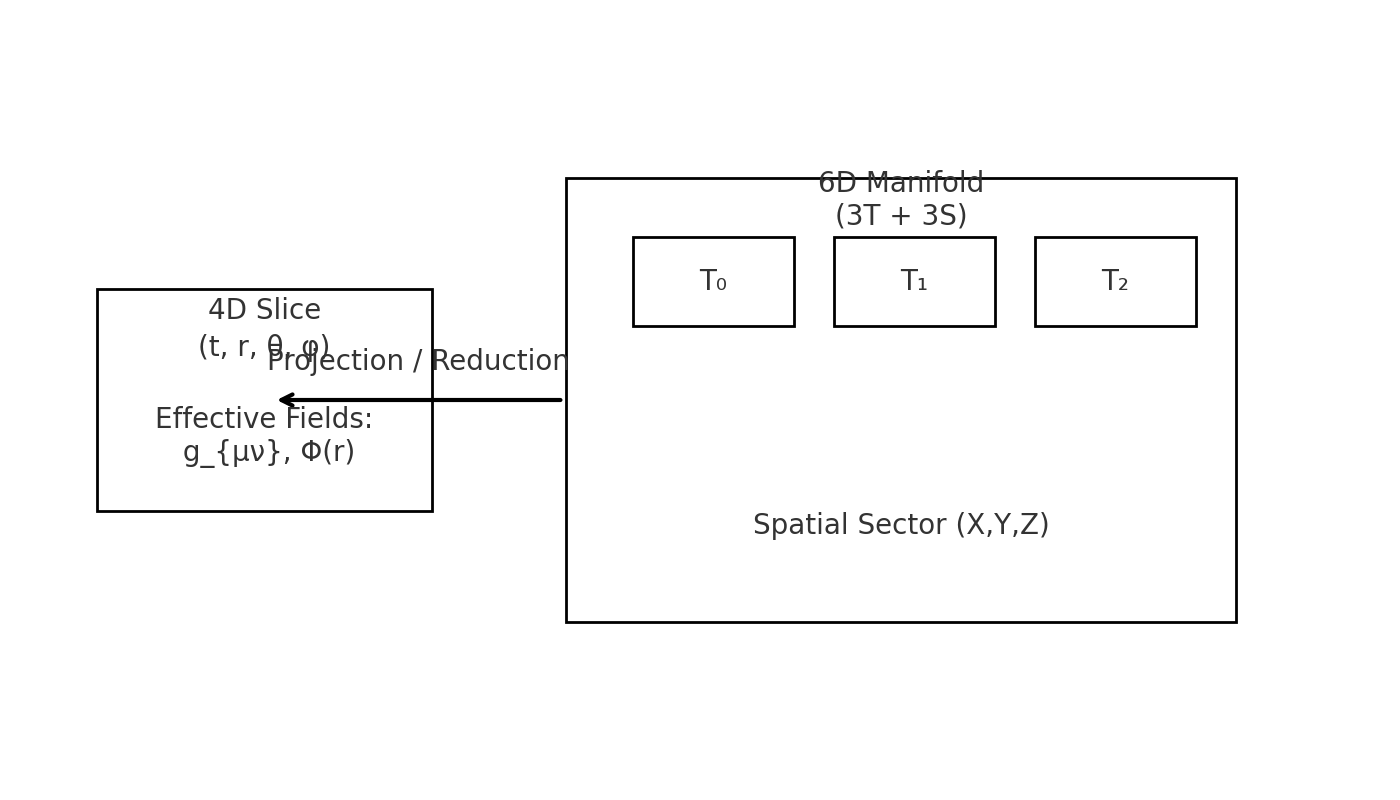
\includegraphics[width=\linewidth]{figures/fig_projection_6D_to_4D.png}
  \caption{Narrative schematic of the projection from a 6D $(3\mathrm{T}+3\mathrm{S})$ manifold to a 4D lab slice with fields $g_{\mu\nu}$ and $\Phi$.}
\end{figure}

\section{Action and Variation in 6D}
Consider
\begin{equation}
S=\int d^6X\,\sqrt{|G|}\,\Big[\frac{1}{2\kappa_6}R_6 - \frac{1}{2}G^{AB}\partial_A\Phi\,\partial_B\Phi - V(\Phi)\Big] + S_{\rm int}[G,\Phi;\alpha_X,\eta].
\end{equation}
Variations yield Einstein-like equations and a scalar equation with interaction sources:
\begin{align}
\frac{1}{2\kappa_6}\Big(R_{AB}-\tfrac{1}{2}G_{AB}R_6\Big) &= T^{(\Phi)}_{AB} + T^{\rm (int)}_{AB},\\
\Box_6\Phi - V'(\Phi) &= \mathcal{J}_{\rm int}.
\end{align}

\section{Projection to a 4D Effective Sector}
Let $\Pi^A{}_{\mu}$ project to a 4D slice. Define $g_{\mu\nu}=\Pi^A{}_{\mu}\Pi^B{}_{\nu}G_{AB}$ and $\Phi(x^\mu)=\Phi(\Pi x)$. Absorbing measure factors into couplings,
\begin{align}
\frac{1}{2\kappa_4}\Big(R_{\mu\nu}-\tfrac{1}{2}g_{\mu\nu}R\Big) &= T^{(\Phi)}_{\mu\nu} + \Delta T^{\rm (int)}_{\mu\nu},\\
\Box\Phi - \frac{dV_{\rm eff}}{d\Phi} &= \mathcal{J}_{\rm eff}.
\end{align}
A \emph{warp gauge condition} enforces subluminal lab evolution: $u^\mu\partial_\mu\Phi=0$.

\section{Static, Spherically Symmetric Reduction}
In the lab weak-field regime ($A\simeq B^{-1}\simeq 1$) with $\Phi=\Phi(r)$,
\begin{equation}
\frac{1}{r^2}\dv{r}\!\left(r^2 \dv{\Phi}{r}\right) - \frac{dV_{\rm eff}}{d\Phi}=0.
\end{equation}
A compact, smooth solution is well-approximated by
\begin{equation}
\Phi(r)\approx \Phi_0 \exp\!\big(-(r/R)^4\big).
\end{equation}

\begin{figure}[h]
  \centering
  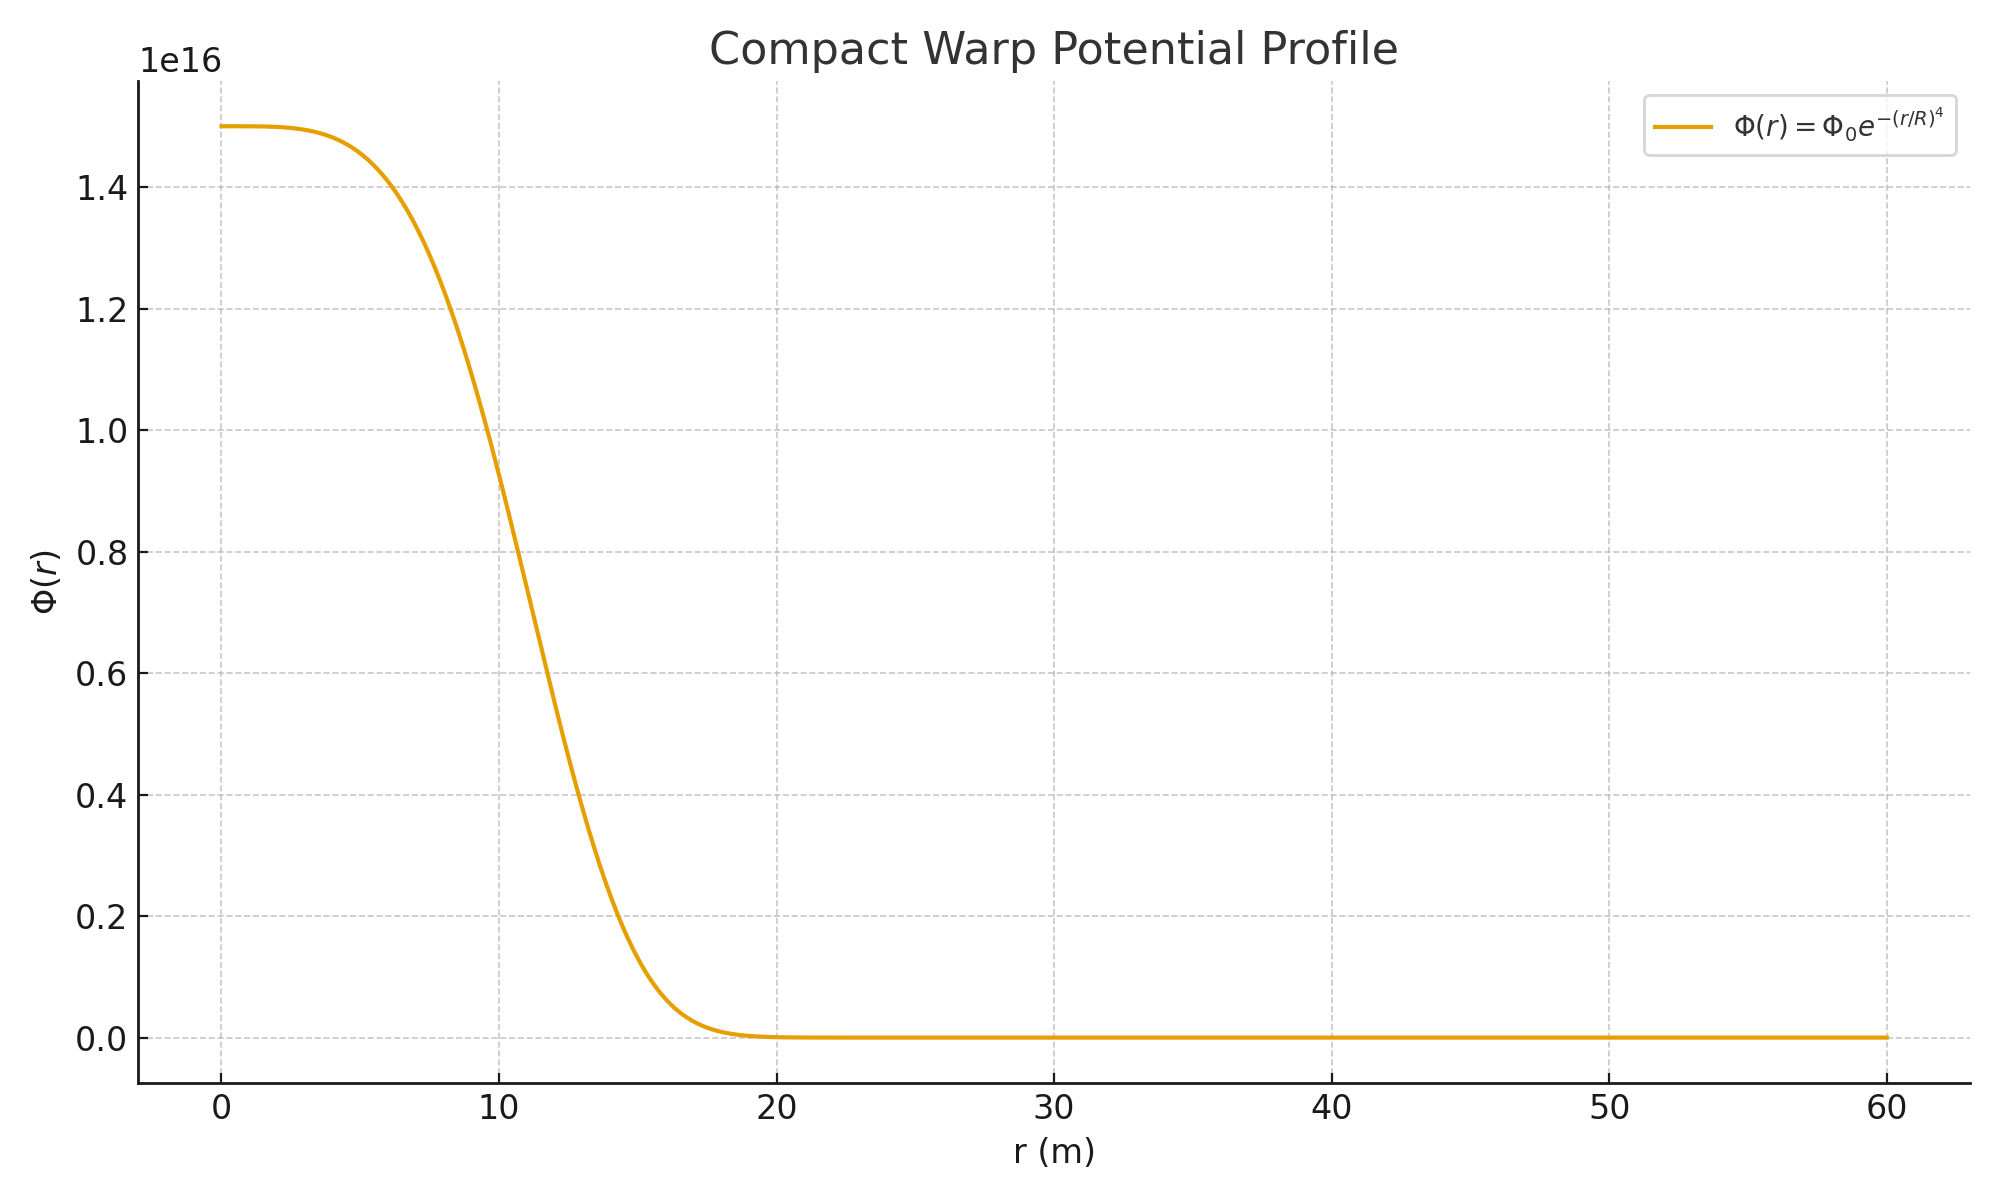
\includegraphics[width=\linewidth]{figures/fig_phi_profile.png}
  \caption{Compact potential profile $\Phi(r)=\Phi_0 e^{-(r/R)^4}$ serving as an analytical ansatz in the weak-field, static limit.}
\end{figure}

\section{Effective Stress--Energy and Curvature}
With $\Phi=\Phi(r)$,
\begin{equation}
\rho_{\rm eff}=\tfrac{1}{2}(\Phi')^2+V_{\rm eff}(\Phi),\qquad p_{\rm eff}=\tfrac{1}{2}(\Phi')^2-V_{\rm eff}(\Phi).
\end{equation}

\begin{figure}[h]
  \centering
  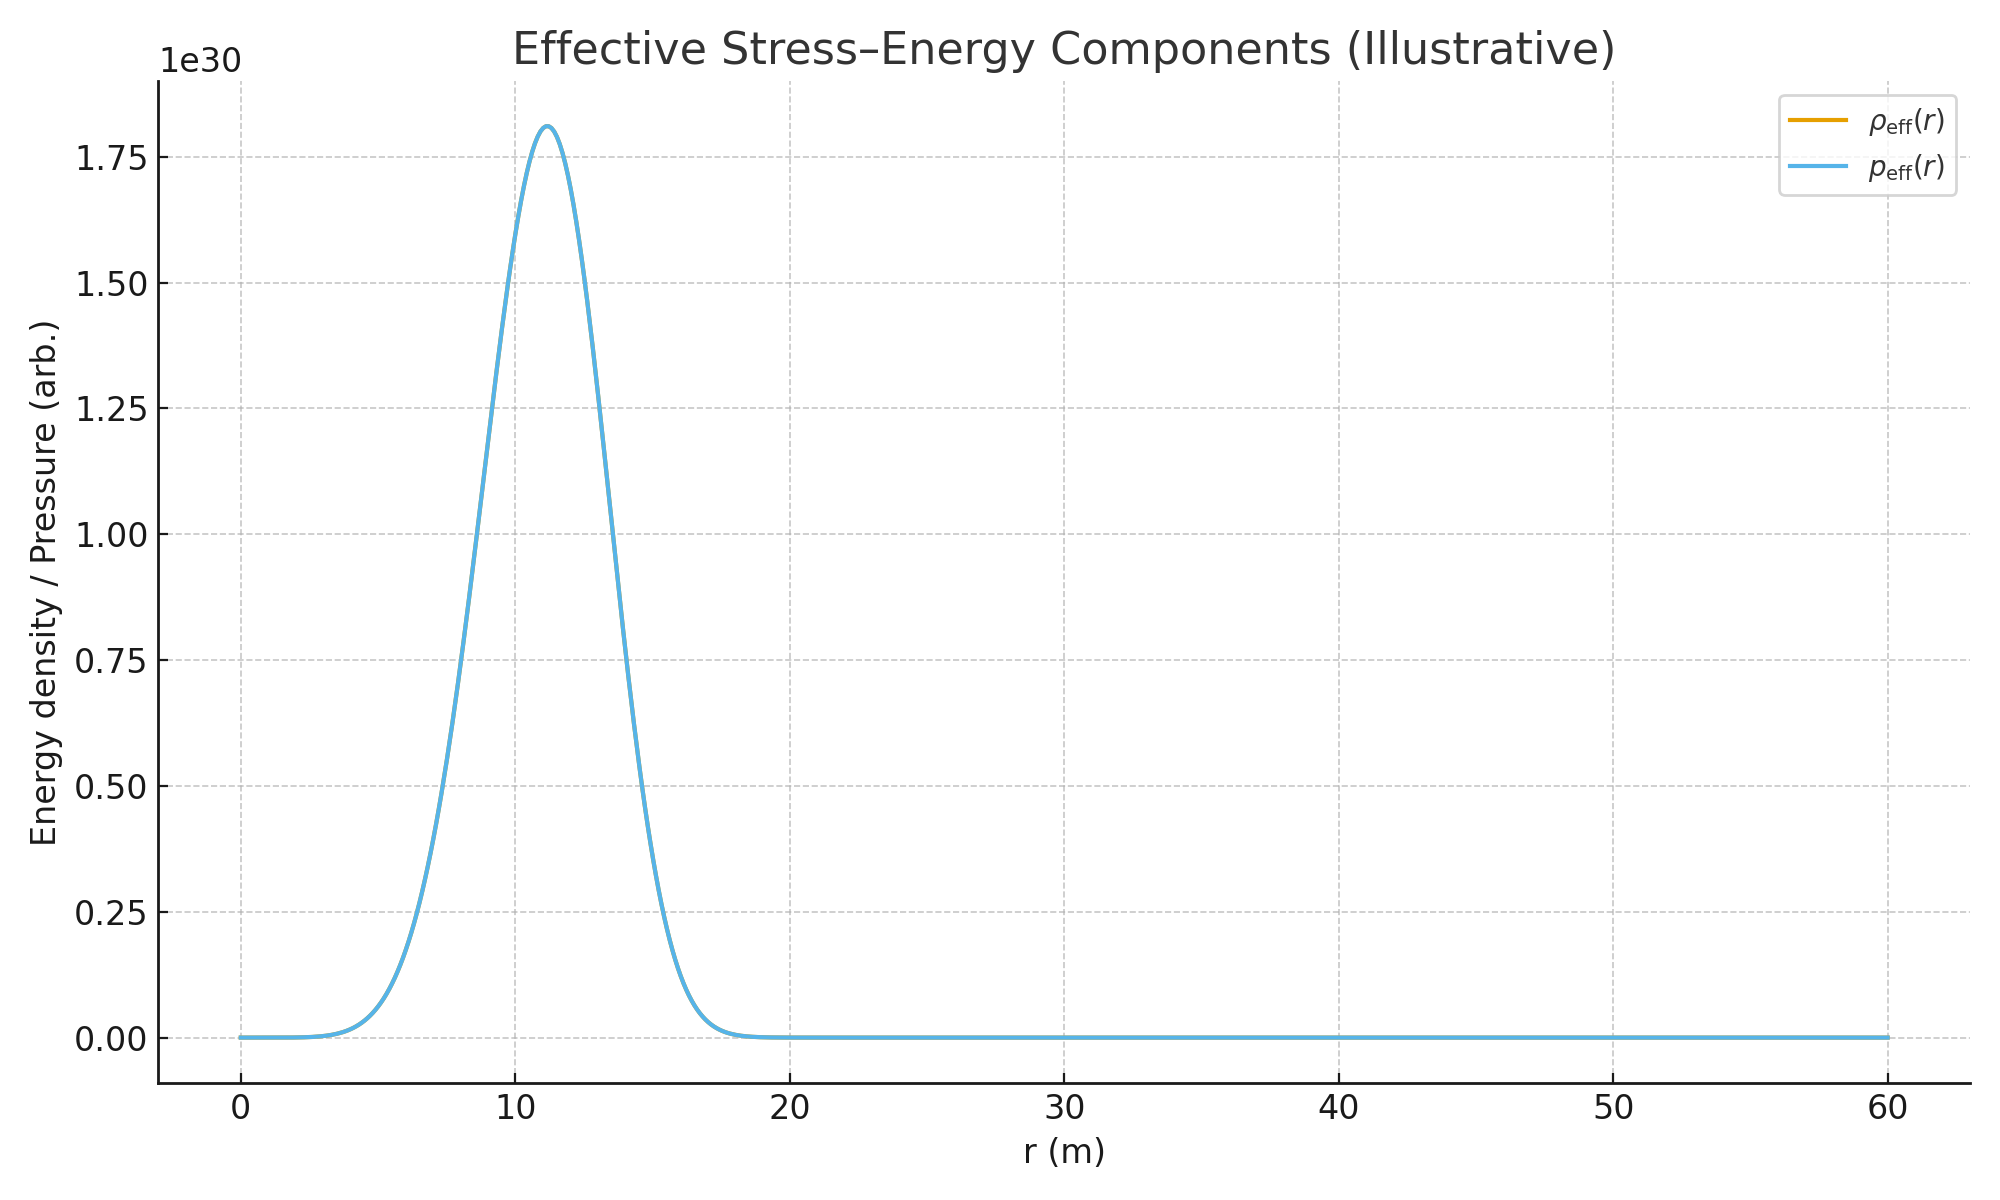
\includegraphics[width=\linewidth]{figures/fig_stress_energy.png}
  \caption{Illustrative effective stress--energy components derived from the compact profile and a simple $V_{\rm eff}(\Phi)$ choice.}
\end{figure}

\section{Mapping to Observables}
First-order metric perturbations yield the laboratory observables used in the toy model:
\begin{align}
\Delta\tau/\tau \simeq \Phi/c^2,\quad
\Delta\phi \simeq \tfrac{4\pi}{\lambda}\Delta L,\quad
\Delta L/L_0 \simeq \beta(\Phi),\quad
g_{\rm eff}\propto -\Phi'(r).
\end{align}

\begin{figure}[h]
  \centering
  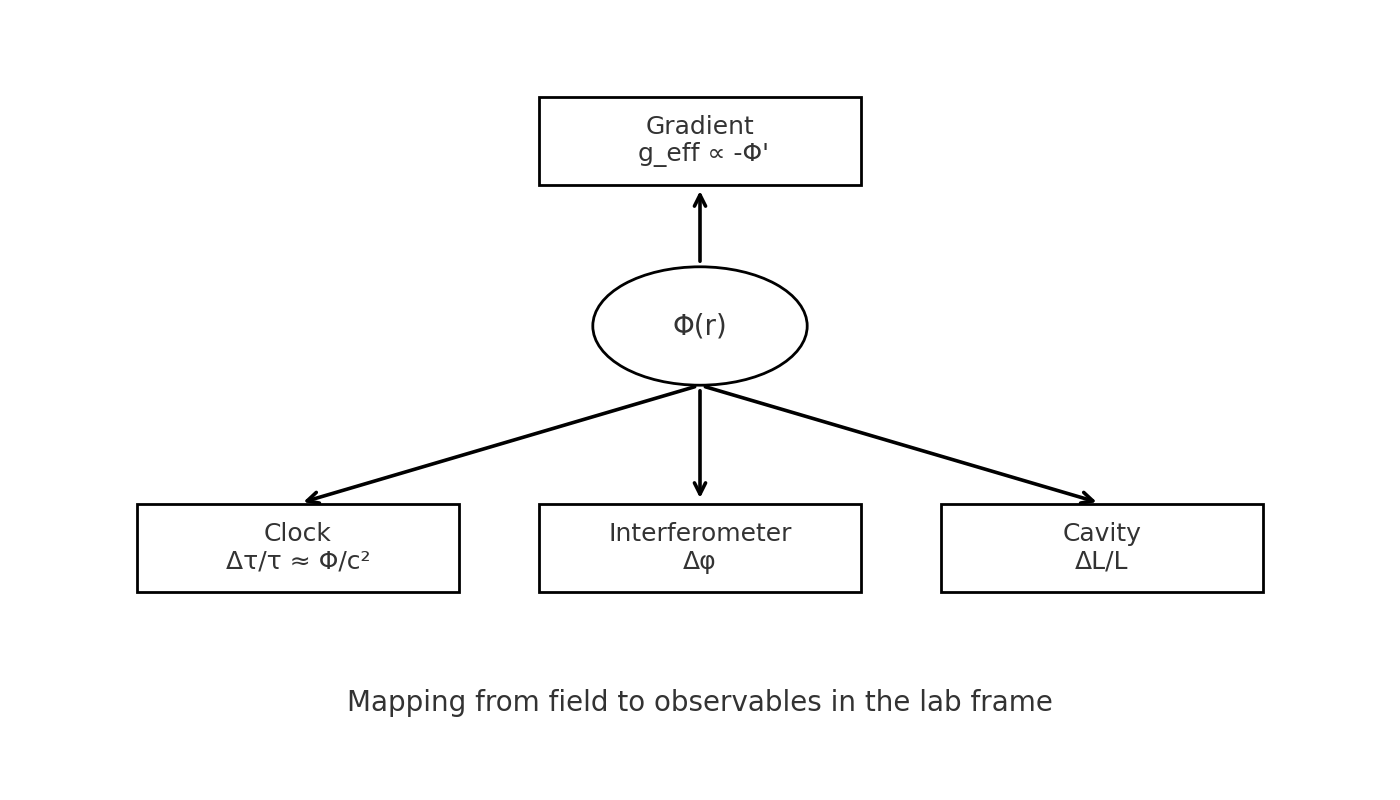
\includegraphics[width=\linewidth]{figures/fig_observable_mapping.png}
  \caption{Narrative mapping from field profile to multimodal observables (clock, interferometer, cavity, gradient).}
\end{figure}

\section*{Conclusions}
We provided a blueprint-to-equations pathway yielding a consistent 4D Einstein--scalar system with a compact warp solution compatible with WLH phenomenology. Constants remain symbolic pending blueprint finalization and empirical tests.

\begin{thebibliography}{9}
\bibitem{BGC2025}
The Burren Gemini Collective (2025), \emph{6D Interaction Matrix --- Universe Blueprint}. 
\bibitem{WLH2025}
The Burren Gemini Collective (2025), \emph{Woven Light Hypothesis v20}, Compendium Series.
\end{thebibliography}

\end{document}
